{\par \bigskip \par \color{red} TODO: Bedrijf Emando B.V. inleiden \par \bigskip \par }

\section{Opdracht samenvatting}
In de weken voorafgaand aan het bachelorproject is in samenspraak met Emando de opdrachtomschrijving gemaakt. Bij het brainstormen zijn de minimale eisen en de mogelijke extra functies bedacht. In de opdracht 

\begin{quotation}
\itshape
Het ontwerpen en ontwikkelen van een systeem voor het weergeven en analyseren van (live) recreatieve en trainingsdata in de context van baansporten (bijvoorbeeld schaatsen en baanwielrennen). Dit systeem zal realtime gegevens van de baan, maar ook opgeslagen gegevens uit het verleden, inzichtelijk maken voor sporters, coaches en eventuele toeschouwers (volgers). Daarnaast zal er de mogelijkheid zijn om een sociale component en een competitie element toe te voegen, en een mogelijkheid om aggregatie op data uit te voeren.

Het systeem ondersteunt het sporten: sporters hoeven hun training niet te onderbreken, doordat audio-cue's en sport-specifieke schermen geïmplementeerd worden. De sociale component bestaat uit het volgen van vrienden (mede-sporters) en het delen van resultaten. Het competitie element zal een virtuele competitie tussen vrienden omvatten.

Technisch gezien zal er een scheiding gemaakt worden tussen de diverse toepassingen (clients) en de API. De API biedt toegang tot realtime data en de diverse modulaire (sport-specifieke) aggregaties, waarbij de mogelijkheid bestaat voor bijvoorbeeld coaches om te abonneren op meerdere sporters. De API zal gekoppeld worden op bestaande systemen die data van transponders ontsluiten.
\end{quotation}

{\par \bigskip \par \color{red} TODO: Formele omschrijving uitleggen \par \bigskip \par }

\section{Reeds bestaande vergelijkbare systemen}

Er bestaan al enkele oplossingen die functionaliteit bieden die vergelijkbaar is met die van de applicatie die wij gaan bouwen. Strava (Figuur~\ref{fig:strava}) en RunKeeper (Figuur~\ref{fig:runkeeper}) maken gebruik van GPS om onderandere hardlopers en wielrenners van realtime informatie te voorzien. MyLaps Practice (Figuur~\ref{fig:mylapspractice}) is een website waar je na je training je prestaties kan terugkijken. Er bestaat ook een iPhone App voor MyLaps Practice (Figuur~\ref{fig:mylapspractice-app}). Coach Watch (Figuur~\ref{fig:coachwatch}) is een iPad applicatie waarmee coaches hun teams kunnen volgen.

\begin{figure}[ht]
\centering
\subfigure[Strava]{
    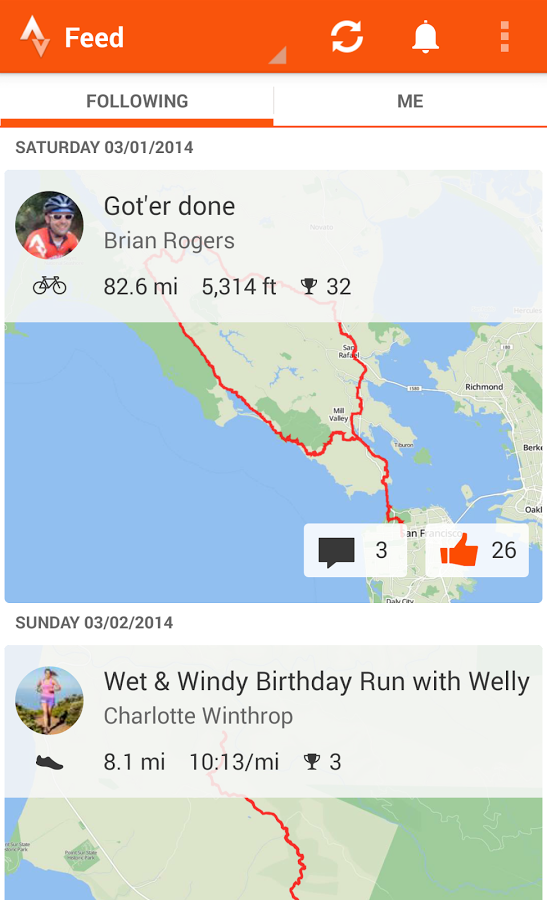
\includegraphics[height=5cm]{style/images/Strava}
    \label{fig:strava}
}
\subfigure[RunKeeper]{
    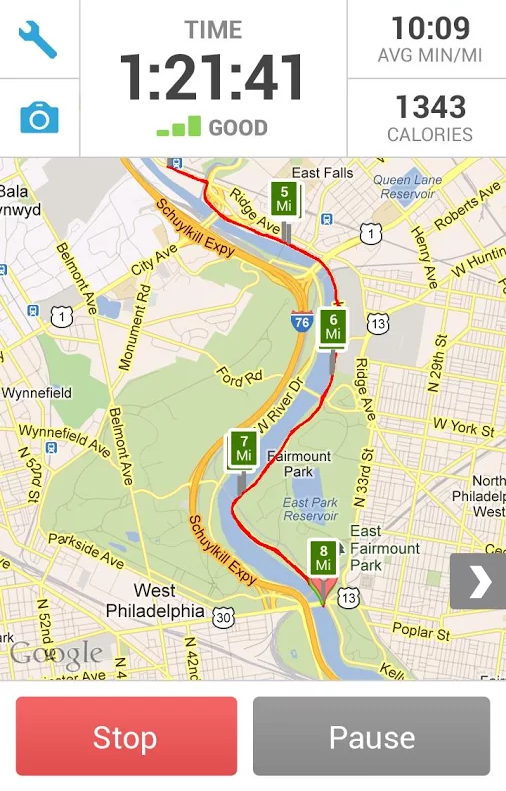
\includegraphics[height=5cm]{style/images/RunKeeper}
    \label{fig:runkeeper}
}
\subfigure[Coach Watch]{
    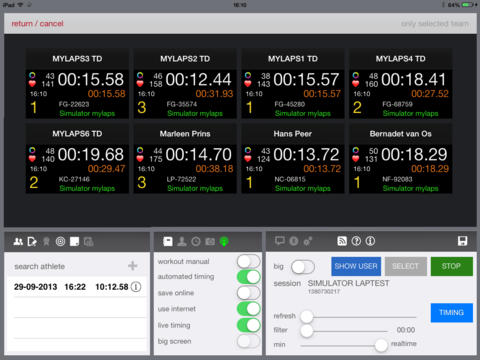
\includegraphics[height=5cm]{style/images/CoachWatch}
    \label{fig:coachwatch}
}

\subfigure[MyLaps Practice]{
    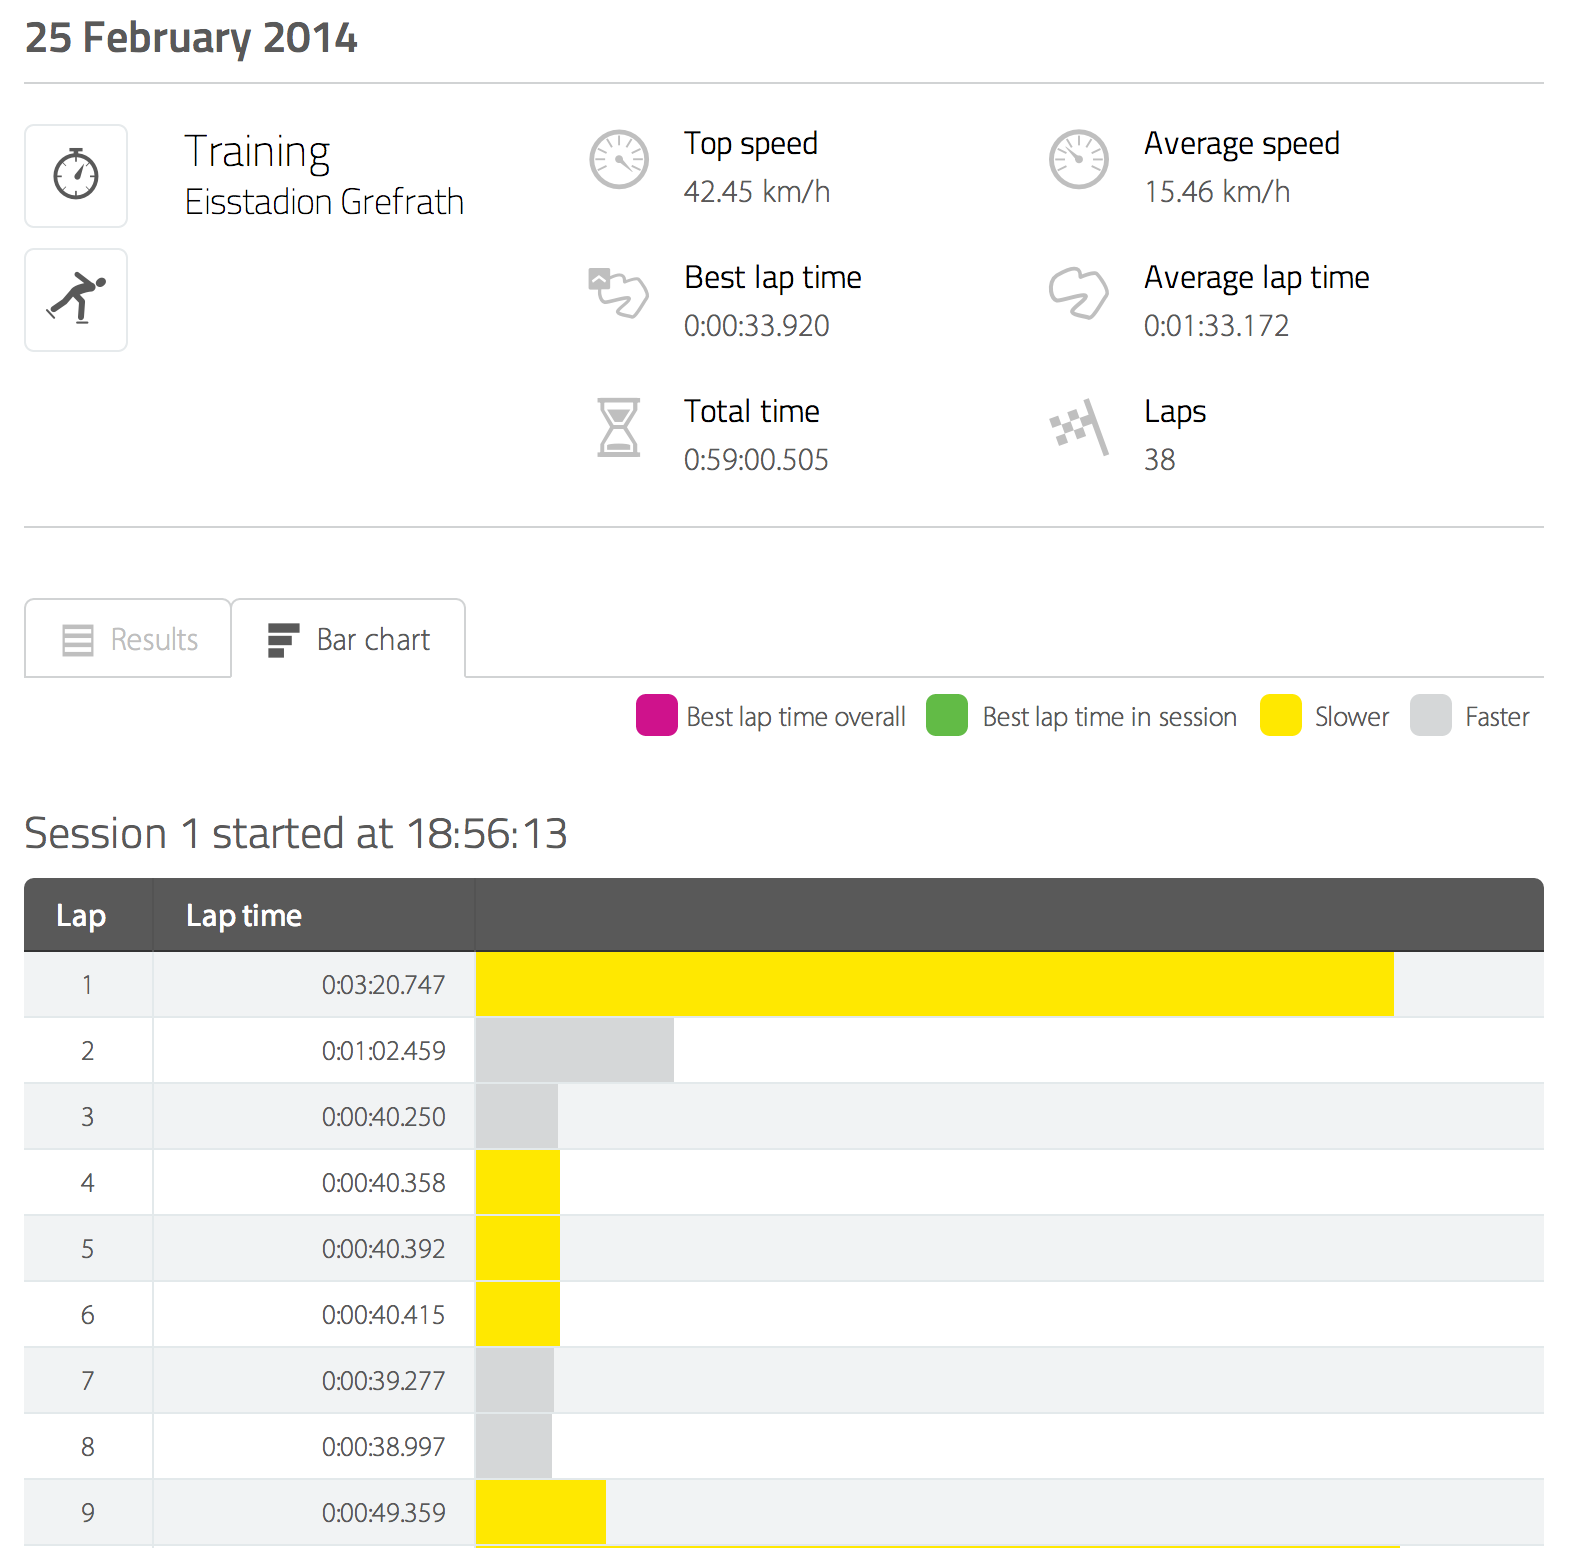
\includegraphics[height=7cm]{style/images/MyLapsPractice}
    \label{fig:mylapspractice}
}
\subfigure[MyLaps Practice App]{
    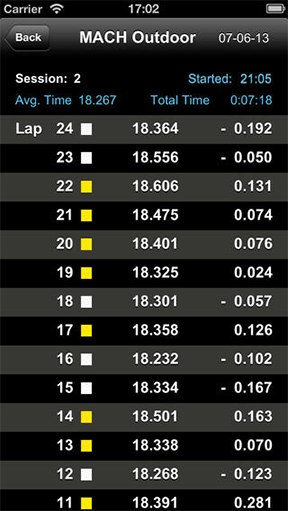
\includegraphics[height=7cm]{style/images/MyLapsPractice-App}
    \label{fig:mylapspractice-app}
}

\caption{Soortgelijke oplossingen}
\label{fig:soortgelijke-oplossingen}
\end{figure}

Strava en RunKeeper zijn voor baansporten, zoals bijvoorbeeld schaatsen, niet goed bruikbaar, aangezien GPS op de banen slecht presteert, waardoor de informatie niet nauwkeurig goenoeg is. MyLaps Practice en Coach Watch maken wel gebruik van de detectielussen in de banen. MyLaps Practice kan alleen gebruikt worden voor het achteraf bekijken van sportprestaties en CoachWatch is een (vrij dure) applicatie die vooral gericht is op coaches.

Emando ziet de mogelijkheid om een applicatie te bieden die gebruikmaakt van de detectielussen in de banen, live gegevens kan tonen op een smartphone en ook nog eens goedkoop of gratis is. Onze applicatie richt zich dus op het invullen van de stukken die missen in de bestaande oplossingen.

    % MyLaps platform
    % KNSB tools: wedstrijdinschrijvings-, tijdregistratie-, SARA-systeem
    % - inschrijven.knsb.nl
    % - oude DOS/XP software
    % - tijden.knsb.nl
    % - schaatscoach.nl (Johan 2008)
    % - osta.nl (Haarlem 2005)
    % KNWU uitslagen op eigen website: (verder uitzoeken)
    % bv. http://www.knwu.nl/baanwielrennen/wedstrijdkalender/evenement/108061
    
    % systemen in ontwikkeling bij Emando
\section{Programma van eisen} % MoSCoW shizzle

{\par \bigskip \par \color{red} TODO: Programma van Eisen overnemen \par \bigskip \par }